
\chapter[A proof of termination, using epsilon0]{A proof of termination, using ordinals below \texorpdfstring{$\epsilon_0$}{epsilon0}}

\label{cnf-math-def}
\label{chap:proof-term}
\label{chap:T1}

In this chapter, we adapt to \coq{} the well-known~\cite{KP82}  proof that Hercules eventually wins every battle, whichever the strategy  of each player.
In other words, we present  a formal and self contained proof of termination  of all [free] hydra battles.
First, we take from Manolios and Vroon~\cite{Manolios2005} a representation of the ordinal $\epsilon_0$ as terms in Cantor normal form. Then, we define a variant for hydra battles as a measure that maps any hydra to some ordinal strictly less than $\epsilon_0$.



\section{The ordinal \texorpdfstring{\(\epsilon_0\)}{epsilon0}}
\label{sec:epsilon0-intro}

\subsection{Cantor normal form}





The ordinal \(\epsilon_0\) is the least ordinal number that satisfies 
the equation \(\alpha = \omega^\alpha\), where \(\omega\) is 
the least infinite ordinal. Thus, we can consider \(\epsilon_0\) as an
\emph{infinite} \(\omega\)-tower.

\index{Maths!Cantor normal form}

Any ordinal strictly less that \(\epsilon_0\) 
can be represented by a unique  \emph{Cantor normal form}, 
that is, an expression  which is either  the ordinal \(0\) or 
a sum  \(\omega^{\alpha_1} \times n_1 + \omega^{\alpha_2} \times n_2 + 
  \dots + \omega^{\alpha_p} \times n_p\) where all the \(\alpha_i\) 
are ordinals in Cantor  normal form, \(\alpha_1 > \alpha_2 > \alpha_p\), 
and all the \(n_i\) are positive integers.

An example of Cantor normal form is displayed in Fig \ref{fig:cnf-example}:
Note that  any ordinal of
the form \(\omega^0 \times i + 0\) is just written \(i\).

\begin{figure}[htb]
\centering
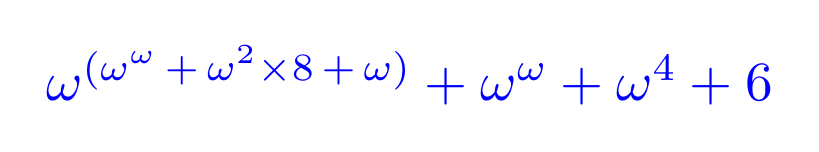
\begin{tikzpicture}[scale=2, every node/.style={transform shape}]
\node[color=blue]{$\omega^{(\omega^\omega\,+\, \omega^2 \times 8 \,+\, \omega)}+ \omega^\omega + \omega^4+ 6$};
\end{tikzpicture}
\caption{\label{fig:cnf-example}
An ordinal in Cantor normal form}
\end{figure}




In the rest of this section, we define an inductive type for representing in \texttt{Coq}
all the ordinals strictly  less than  \(\epsilon_0\), then extend some arithmetic operations
to this type, and finally prove that our representation fits well with 
the expected mathematical properties: the order we define is a well order, 
and the decomposition into Cantor normal form  is consistent 
with the implementation of the arithmetic operations of exponentiation of base \(\omega\) 
and addition.

\paragraph*{Remark}
\label{sec:orgheadline65}
Unless explicitly mentionned, the term ``ordinal" will be used instead of
``ordinal strictly less than \(\epsilon_0\)" (except in Chapter~\ref{chap:schutte} where it stands for ``countable ordinal'').



\subsection{A data type for  ordinals in Cantor normal form}
\label{sec:orgheadline72}
\label{sec:T1-inductive-def}



% Our user contribution~\cite{CantorContrib} represents 
% the set of ordinals strictly less than $\epsilon_0$ in Cantor normal form as in~\cite{Manolios2005}, and also the set
% of ordinals strictly  less than $\Gamma_0$ in Veblen normal form.


    Let us define an inductive type whose 
constructors are respectively associated
with the ways to build Cantor normal forms:

\begin{itemize}
\item the ordinal \(0\)
\item the construction \((\alpha,\, n,\,\beta)  \mapsto \omega^\alpha \times (n + 1)+ \beta \quad (n\in\mathbb{N})\)
\end{itemize}


\vspace{4pt}
\noindent\emph{From Module~\href{../src/html/hydras.Epsilon0.T1.html\#T1}{Epsilon0.T1}}

\index{Types!T1@T1 (ordinal terms below $\epsilon_0$)}
\index{Constants!zero:T1}


\begin{Coqsrc}
Inductive T1 : Set  :=
| zero : T1
| ocons : T1 -> nat -> T1 -> T1.
\end{Coqsrc}



\subsubsection*{Remark}
\label{sec:orgheadline66}


The name \texttt{T1} we gave to this data-type  is proper to this development and refers
to a hierarchy of ordinal notations. For instance, in~\cite{CantorContrib}, the following type is used to represent ordinals strictly less than \(\Gamma_0\),  in Veblen normal form (see also~\cite{schutte}).

\index{Types!T2@T2 (ordinals in Veblen normal form)}
\emph{Please look also at sub-directory
href{../src/html/hydras.Gamma0.T2.html}{Gamma0.T2.html}}.


\begin{Coqsrc}
Inductive T2 : Set :=
  zero : T2
| gcons : T2 -> T2 -> nat -> T2 -> T2.
\end{Coqsrc}

Another useful ordinal notation could be used for denoting the ordinals strictly less than $\omega^\omega$, but \texttt{list nat} could be used as well.

\begin{Coqsrc}
Inductive T0 : Set := 
  zero : T0
| cons : nat -> T0 -> T0.
\end{Coqsrc}


\subsubsection{Example}

\label{alpha0-def}
For instance, the ordinal  $\omega^\omega+\omega^3\times 5+2$ is represented by the following term:

\begin{Coqsrc}
Example alpha_0 : T1 :=
  ocons (ocons (ocons zero 0 zero)
               0
               zero)
        0
       (ocons (ocons zero 2 zero)
              4
              (ocons zero 1 zero)).
\end{Coqsrc}


\begin{figure}[htb]
\centering
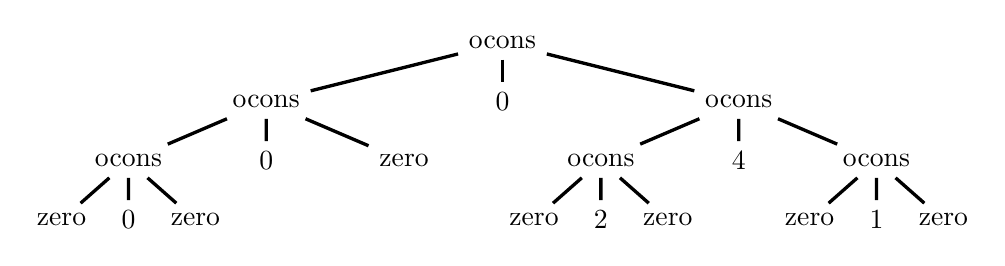
\begin{tikzpicture}[very thick, scale=0.5, level 1/.style={sibling distance=6cm},
level 2/.style={sibling distance=35mm},  
level 3/.style={sibling distance=17mm}]
\node  {ocons}
  child {  node {ocons}
            child { node {ocons} child {node {zero}} child {node{0}} child{node{zero}}}
         child {node {0}}
         child {node {zero}}}
    child {node {0}}
   child {node {ocons} 
 child { node {ocons} child {node {zero}} child {node{2}} child{node{zero}}}
  child {node {4}}
         child {node {ocons} child {node {zero}} child {node{1}} child{node{zero}}}};

\end{tikzpicture}

\caption{The tree-like representation of the ordinal $\omega^\omega+\omega^3\times 5 +2$\label{fig:cnf-tree}}

\end{figure}



\paragraph{Remark}
For simplicity's sake, we chosed to forbid  expressions of the form $\omega^\alpha\times 0 + \beta$. Thus, the contruction (\texttt{ocons $\alpha$ $n$ $\beta$} is intented to represent the
ordinal $\omega^\alpha\times(n+1)+\beta$ and not $\omega^\alpha\times n+\beta$.
In a future version, we should replace  the type \texttt{nat} with \texttt{positive} in \texttt{T1}'s 
definition. But this replacement would take a lot of time \dots.

\subsection{Abbreviations}

Some abbreviations may help to write more consisely complex ordinal terms.

\subsubsection{Finite ordinals}
\label{sec:orgheadline67}

For representing finite ordinals, \emph{i.e.} natural numbers, we first introduce a notation for terms of the form $n+1$, then define a coercion from type \texttt{nat} into \texttt{T1}.

\begin{Coqsrc}
Notation "'FS' n" :=
     (ocons zero n zero) (at level 10) : t1_scope.
\end{Coqsrc}

\begin{Coqsrc}
Definition fin (n:nat) : T1 := 
    match n with 0 => zero | S p => FS p end.

Coercion fin  : nat >-> T1.

Example ten : T1 := 10.   
\end{Coqsrc}

\index{Coq!Techniques!Coercions}
\index{Functions!Coercions@Coercions (from nat to ordinal types)}
\begin{remark}
\label{warning:coercions}
The use of coercions like \texttt{fin} allow us to be close to the mathematical tradition where natural numbers are ordinals too.
Nevertheless, it may happen that a goal like \texttt{3 < 5} could be 
interpreted as \texttt{(lt (fin 3) (fin 5))},  depending on the current notation scope.  
When this misinterpretation happens, tactics like \texttt{auto with arith}, \texttt{lia} do not work!
Thus, it is useful to write \texttt{(3 < 5)\%nat}  an inequality between two natural numbers. 
\end{remark}


\subsubsection{The ordinal \(\omega\)}
\label{sec:orgheadline68}

  Since \(\omega\)'s Cantor normal form is
i.e. \(\omega^{\omega^0}\times 1+ 0\), we can define the following abbreviation:

\index{Notations!omega@omega (the least infinite ordinal)}
\begin{Coqsrc}
Notation omega := (ocons (ocons zero 0 zero) 0 zero).
\end{Coqsrc}

Note that \texttt{omega} is not an identifier, thus any tactic like \texttt{unfold omega} would fail.


\subsubsection{The ordinal \(\omega^\alpha\), a.k.a. \(\varphi_0(\alpha)\)}
\label{sec:orgheadline70}

We provide also a notation for ordinals of the form $\omega^\alpha$.

\index{Notations!phi0@phi0 (exponential of base omega)}

\begin{Coqsrc}
Notation "'phi0' alpha" := (ocons alpha 0 zero) (at level 29) : t1_scope.
\end{Coqsrc}

\index{Maths!Additive principal ordinals}

\begin{remark}
\label{sec:orgheadline69}
The name \(\varphi_0\)
   comes from ordinal numbers theory. In~\cite{schutte}, Schütte defines 
$\varphi_0$  as the ordering (\emph{i.e.} enumerating) function of the set  of \emph{additive principal ordinals} \emph{i.e.} strictly positive ordinals $\alpha$ that verify $\forall \beta<\alpha, \beta+\alpha=\alpha$. For Schütte,  $\omega^\alpha$ is just a notation for $\varphi_0(\alpha)$.  See also Chapter~\vref{chap:schutte}.
\end{remark}



  
\subsubsection{The hierarchy of \(\omega\)-towers:}
\label{sec:orgheadline71}

The ordinal $\epsilon_0$, although not represented by a finite term in Cantor normal form, is approximed by the sequance of $\omega$-towers.

\vspace{4pt}
\emph{From Module~\href{../src/html/hydras.Epsilon0.T1.html}{Epsilon0.T1}}

\begin{Coqsrc}
Fixpoint omega_tower (height:nat) : T1 := 
 match height with 
 | 0 =>  1 
 | S h => phi0 (omega_tower h)
 end.
\end{Coqsrc}

For instance, Figure~\ref{fig:tower7} represents  the ordinal returned by the
 evaluation of the term \texttt{omega\_tower 7}.

\begin{figure}[htb]
\centering
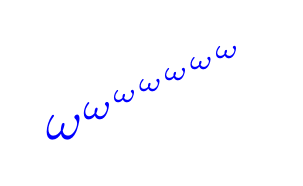
\begin{tikzpicture}[scale=2, every node/.style={transform shape}]
\node[color=blue]{$\omega^{{{\omega}^{{{\omega}}^{{{\omega}}^{{\omega^{{\omega}^{\omega}}}}}}}}$};
\end{tikzpicture}
\caption{\label{fig:tower7}
The $\omega$-tower of height 7}
\end{figure}



\subsection{Comparison between ordinal terms}
\label{sec:orgheadline73}


% Our formalisation of Cantor Normal Form will take two steps:
% 1 Definition of a strict order \texttt{<} on the type \texttt{T1}, 
% 2 Using \texttt{<} for characterizing terms in normal form.

In order to compare two terms of type \texttt{T1}, we define a recursive function \texttt{compare} that maps two ordinals $\alpha$ and $\beta$ to a value of type \texttt{comparison}. This type is defined in \coq's standard library 
\texttt{Init.Datatypes} and
contains three constructors:  \texttt{Lt} (less than), \texttt{Eq} (equal), and
\texttt{Gt} (greater than).


\vspace{4pt}
\emph{From Module~\href{../src/html/hydras.Epsilon0.T1.html\#compare}{Epsilon0.T1}}


\begin{Coqsrc}
Fixpoint compare (alpha alpha':T1):comparison :=
  match alpha, alpha' with
    zero, zero => Eq
  | zero, ocons a' n' b' => Lt
  | _   , zero => Gt
  | (ocons a n b),(ocons a' n' b') =>
      (match compare a a' with 
          | Lt => Lt
          | Gt => Gt
          | Eq => (match lt_eq_lt_dec n n'
                   with
                       inleft  (left _) => Lt
                     | inright _ => Gt
                     |   _ => compare b b'
                   end)
       end)
  end.
\end{Coqsrc}
 
It is now easy to define the boolean predicate \texttt{lt\_b $\alpha$ $\beta$}: 
`` $\alpha$ is strictly less than $\beta$ ''. By coercion to sort \texttt{Prop} we define also the predicate \texttt{lt}.

\vspace{4pt}
\emph{From Module~\href{../src/html/hydras.Epsilon0.T1.html}{Epsilon0.T1}}


\begin{Coqsrc}
Definition lt_b alpha beta : bool :=
  match compare alpha beta with
      Lt => true
    | _ => false
  end.

Definition lt alpha beta : Prop := lt_b alpha beta.
\end{Coqsrc}

\index{Predicates!lt @ lt (total, strict, non-well founded order on type T1)}
Please note that this definition of \texttt{lt} makes it easy to write proofs by reflection, as shown by the following examples.

\begin{Coqsrc}
Example E1 : lt (ocons omega 56 zero) (tower 3).
Proof. reflexivity. Qed.

Example E2 : ~ lt (tower 3) (tower 3).
Proof.  discriminate.  Qed.
\end{Coqsrc}

The following lemmas establish relations between \texttt{compare}, 
the predicate \texttt{lt} and Leibniz equality \texttt{eq}.

\vspace{4pt}
\emph{From Module~\href{../src/html/hydras.Epsilon0.T1.html\#compare_refl}{Epsilon0.T1}}


\begin{Coqsrc}
Lemma compare_refl : forall alpha, compare alpha alpha =  Eq.
\end{Coqsrc}

\begin{Coqsrc}
Lemma compare_reflect : forall alpha beta,
    match compare alpha beta with
    |   Lt => lt alpha  beta
    |   Eq => alpha = beta
    |   Gt => lt beta  alpha
    end.
\end{Coqsrc}

We prove also that the relation \texttt{lt} is a strict total order.

\vspace{4pt}
\emph{From Module~\href{../src/html/hydras.Epsilon0.T1.html\#lt_irrefl}{Epsilon0.T1}}

  
\begin{Coqsrc}
Theorem lt_irrefl : forall alpha, ~ lt alpha  alpha.

Theorem lt_trans :
forall alpha beta: T1,
 lt alpha  beta -> 
 forall gamma, lt beta gamma -> lt alpha gamma.

Definition lt_eq_lt_dec  :
   forall alpha beta : T1, 
          {lt alpha  beta} + {alpha = beta} + {lt beta alpha}.
\end{Coqsrc}


Note that the order \texttt{lt} is not reflected 
in the structure (size and/or height) of the terms of \texttt{T1}. 
For instance the ordinal of Fig \ref{fig:cnf-example} is strictly less
than the structurally simpler \(\omega^{\omega^\omega}\times 2\).

\subsubsection{A Predicate for characterizing normal forms}
\label{sec:orgheadline74}
\label{sec:orgheadline75}
We note that our data-type \texttt{T1} allows us to write expressions that
are not properly in Cantor normal form as specified in Section \ref{sec:epsilon0-intro}.
For instance, consider the following term of type  \texttt{T1}. 

\begin{Coqbad}
Example bad_term  : T1 := ocons 1 1 (ocons omega 2 zero).
\end{Coqbad}

This term would have been written \(\omega^1\times 2 + \omega^\omega \times 3\) in the usual mathematical notation. We note that the exponents of $\omega$ are not in the right (strictly decreasing) order.

With the help of the order \texttt{lt} on \texttt{T1}, we are now able to characterize
the set of all well-formed ordinal terms:


\vspace{4pt}
\emph{From Module~\href{../src/html/hydras.Epsilon0.T1.html\#nf_b}{Epsilon0.T1}}

\index{Predicates!nf @ nf (being in Cantor normal form)}

\begin{Coqsrc}
Fixpoint nf_b (alpha : T1) : bool :=
  match alpha with
    | zero => true
    | ocons a n zero => nf_b a
    | ocons a n ((ocons a' n' b') as b) =>
      (nf_b a && nf_b b && lt_b a' a)%bool
  end. 

Definition nf alpha :Prop := nf_b alpha.
\end{Coqsrc}

\begin{Coqsrc}
 Compute nf_b alpha_0.
\end{Coqsrc}

\begin{Coqanswer}
   = true 
     : bool
\end{Coqanswer}

\begin{Coqsrc}
 Compute nf_b bad_term.
\end{Coqsrc}

\begin{Coqanswer}
   = false 
     : bool
\end{Coqanswer}



\subsection{Making normality implicit}
  We would like to get rid of terms of type \texttt{T1} which are not in Cantor normal form.
A simple way to do this is to consider statements of the form 
\texttt{forall alpha: T1, nf alpha -> $P$ alpha}, where $P$ is a predicate over type \texttt{T1}, lile in the following lemma.

\begin{Coqsrc}
Lemma plus_is_zero alpha beta :
  nf alpha -> nf beta ->
  alpha + beta  = zero -> alpha = zero /\  beta = zero.
\end{Coqsrc}

But this style leads to clumsy statements, and many sub-goals in interactive proofs (although often solved with \texttt{auto} or \texttt{eauto}).

Another way is encapsulate conditions of the form \texttt{(nf $\alpha$)} in
often used predicates. For instance, we introduced the restriction of \texttt{lt} to terms in normal form, and provided a handy notation for this restriction.

\vspace{4pt}
\emph{From Module~\href{../src/html/hydras.Prelude.Restriction.html}{Ordinals.Prelude.Restriction}}

\begin{Coqsrc}
Definition restrict {A:Type}(E: Ensemble A)(R: relation A) :=
    fun a b => E a /\ R a b /\ E b.
 \end{Coqsrc}

 
\vspace{4pt}
\emph{From Module~\href{../src/html/hydras.Epsilon0.T1.html\#LT}{Epsilon0.T1}}

\begin{Coqsrc}
Definition LT := restrict nf lt.
Infix "<" := LT : t1_scope.

Definition LE := restrict nf le.
Notation "alpha <= beta" := (LE alpha beta) : t1_scope.
\end{Coqsrc}

\index{Predicates!LT @LT (partial, well-founded strict order on type T1)}


For instance, in the following lemma, the condition that $\alpha$ is in normal form is included in the condition $\alpha< 1$.

\begin{Coqsrc}
Lemma LT_one : forall alpha, alpha < one -> alpha = zero.
\end{Coqsrc}

  
\subsection{A first-class type for \texorpdfstring{$\epsilon_0$}{epsilon0}}

In Sect~\vref{sect:equations}, we chosed to define total functions over the set of ordinals less than $\epsilon_0$, using M. Sozeau's plug-in
\texttt{coq-equations}\cite{sozeau:hal-01671777}.

To this end, we define a type for representing terms in Cantor normal form,
as a \coq{} type-class.

\label{sect:E0-def}
\index{Types!E0@ EO (ordinal terms below $\epsilon_0$ in normal form)} 

\emph{From Module~\href{../src/html/hydras.Epsilon0.E0.html}{Epsilon0.E0}}

\index{Coq!Techniques!Type classes}

\begin{Coqsrc}
Class E0 : Type := t1_2o {cnf : T1; cnf_ok : nf cnf}.
\end{Coqsrc}

Many constructs : types, predicates, functions, notations, etc., on type \texttt{T1} are adapted to \texttt{E0}.

First, we declare a notation scope for \texttt{E0}.

\begin{Coqsrc}
Declare Scope E0_scope.
Delimit Scope E0_scope with e0.
Open Scope E0_scope.
\end{Coqsrc}

Then we redefine the predicates of comparison.

\index{Predicates!Lt @ Lt (Total, strict, well-founded order on type E0)}

\begin{Coqsrc}
Definition Lt (alpha beta : E0) := T1.LT (@cnf alpha) (@cnf beta).
Definition Le (alpha beta : E0) := T1.LE (@cnf alpha) (@cnf beta).

Infix "<" := Lt : E0_scope.
Infix "<=" := Le : E0_scope.
\end{Coqsrc}
  


Equality in \texttt{E0} is just Leibniz equality. Note that, since \texttt{nf} is
defined by a Boolean function, for  any term $\alpha:\texttt{T1}$, there exists at most one proof of \texttt{nf $\alpha$}, thus two ordinals of type \texttt{E0} are
equal if and only iff their projection to \texttt{T1} are equal.

\index{Coq!Techniques!Unicity of  equality proofs}

\begin{Coqsrc}
Require Import Logic.Eqdep_dec.

Lemma nf_proof_unicity :
  forall (alpha:T1) (H H': nf alpha), H = H'.

Lemma E0_eq_iff alpha beta : alpha = beta <-> cnf alpha = cnf beta.
\end{Coqsrc}

For upgrading constants and fonctions of \texttt{T1}, we have to prove that 
the term they build is in normal form.
For instance, let us represent the ordinals $0$ $\omega$ as instances of the class \texttt{E0}.

\index{Notations!omega@omega (the least infinite ordinal)}
\index{Constants!zero:T1}

\begin{Coqsrc}
Instance Zero : E0.
Proof.
  refine (@mkord T1.zero _);  now compute. 
Defined.

Instance _Omega : E0.
Proof.  now exists omega. Defined.

Notation "'omega'"  := _Omega : E0_scope.
\end{Coqsrc}

 Likewise, we define an addition in type \texttt{E0}, using the function{T1.plus}
and its properties.

\begin{Coqsrc}
Search   (nf (_ + _)%t1).
\end{Coqsrc}

\begin{Coqanswer}
plus_nf: forall a : T1, nf a -> forall b : T1, nf b -> nf (a + b)
\end{Coqanswer}

\begin{Coqsrc}
Instance plus (alpha beta : E0) : E0.
Proof.
  refine (@mkord (T1.plus (@cnf alpha) (@cnf beta))_ );
    apply plus_nf; apply cnf_ok.
Defined.

Infix "+" := plus : E0_scope.

Check omega + omega.
\end{Coqsrc}

\begin{Coqanswer}
omega + omega
     : E0
\end{Coqanswer}




\subsection{Syntactic definition of limit and successor ordinals}

Pattern matching and structural recursion allow us to define the notions of successor and limit ordinal with the help of  boolean functions on type \texttt{T1}. 

 \vspace{4pt}
\emph{From Module~\href{../src/html/hydras.Epsilon0.T1.html\#is_succ}{Epsilon0.T1}}

\begin{Coqsrc}
  Fixpoint is_succ alpha :=
  match alpha with
      zero => false
    | ocons zero _ _ => true
    | ocons alpha n beta => is_succ beta
  end.

Fixpoint is_limit alpha :=
  match alpha with
      zero => false
    | ocons zero _ _ => false
    | ocons alpha n zero => true
    | ocons alpha n beta => is_limit beta
  end.
\end{Coqsrc}



\begin{Coqsrc}
  Compute is_limit omega.
\end{Coqsrc}

\begin{Coqanswer}
  = true
     : bool
\end{Coqanswer}

\begin{Coqsrc}
Compute is_succ 42.
\end{Coqsrc}

\begin{Coqanswer}
  = true
     : bool
   \end{Coqanswer}

The correctness of these definitions with respect to the mathematical notions of
limit and successor ordinals is established through several lemmas. For instance,
Lemma \texttt{canonS\_limit}, page~\pageref{lemma:canonS-limit}, shows that
if $\alpha$ is (syntactically) a limit ordinal, then it is the least upper bound of
a strictly increasing sequence of ordinals.





   The following function is very useful in constructions by cases (proofs and function definitions).
   
\begin{Coqsrc}
  Definition zero_succ_limit (alpha: T1) :
  {is_succ alpha} + {is_limit alpha} +  {alpha=zero}.
  (* ... *)
Defined.
 \end{Coqsrc}

\subsection{Arithmetic on \texorpdfstring{$\epsilon_0$}{epsilon0}}
\subsubsection{Successor}

The successor of any ordinal $\alpha< \epsilon_0$ is defined by structural 
recursion on its Cantor normal form.

\index{Functions!T1.succ}

\vspace{4pt}
\emph{From Module~\href{../src/html/hydras.Epsilon0.T1.html\#succ}{Epsilon0.T1}}

\begin{Coqsrc}
Fixpoint succ (alpha:T1) : T1 :=
  match alpha with zero => 1
             | ocons zero n _ => ocons zero (S n) zero
             | ocons beta n gamma => ocons beta n (succ gamma)
 end.
\end{Coqsrc}


The following lemma establishes the connection between the function
\texttt{succ} and the predicate \texttt{is\_succ}.


\begin{Coqsrc}
 Lemma is_succ_iff alpha (Halpha : nf alpha) :
  is_succ alpha <-> exists beta : T1, nf beta /\ alpha = succ  beta.
\end{Coqsrc}


\subsubsection{Addition and multiplication}

Ordinal addition and multiplication are also defined by structural recursion over the type \texttt{T1}. Please note that they use the \texttt{compare} function on some subterms of their arguments.

\begin{Coqsrc}
Fixpoint plus (alpha beta : T1) : T1 :=
  match alpha,beta with
 |  zero, y  => y
 |  x, zero  => x
 |  ocons a n b, ocons a' n' b' =>
    (match compare a a' with
     | Lt => ocons a' n' b'
     | Gt => (ocons a n (plus b (ocons a' n' b')))
     | Eq  => (ocons a (S(n+n')) b')
     end)
  end
where "alpha + beta" := (plus alpha beta) : t1_scope.
\end{Coqsrc}

\begin{Coqsrc}
Fixpoint mult (alpha beta : T1) :T1 :=
  match alpha,beta with
 |  zero, y  => zero
 |  x, zero => zero
 |  ocons zero n _, ocons zero n' _ => 
                 ocons zero (Peano.pred((S n) * (S n'))) zero
 |  ocons a n b, ocons zero n' b' =>  
                 ocons a (Peano.pred((S n) * (S n'))) b
 |  ocons a n b, ocons a' n' b' =>
     ocons (a + a') n' ((ocons a n b) * b')
 end
where  "alpha * beta" := (mult alpha beta) : t1_scope.
\end{Coqsrc}


\subsubsection{Examples}

The following examples are instances of \emph{proofs by computation}. Please note that  addition and multiplication on \texttt{T1}
are not commutative. Moreover,  both operations fail to be strictly monotonous in their first argument.


\begin{Coqsrc}
Example e2 : 6 + omega = omega.
Proof. reflexivity. Qed.

Example e'2 : omega < omega + 6.
Proof. now compute. Qed.

Example e''2 : 6 * omega = omega.
Proof. reflexivity. Qed.

Example e'''2 : omega < omega * 6.
Proof. now compute. Qed.
\end{Coqsrc}

\begin{Coqsrc}
Lemma plus_not_monotonous : exists alpha beta gamma : T1,
    alpha < beta /\ alpha + gamma = beta + gamma.
Proof.
  exists 3, 5, omega;  now  compute.
Qed.

Lemma mult_not_monotonous :  exists alpha beta gamma : T1,
      alpha < beta /\ alpha * gamma = beta * gamma.
Proof.
  exists 3, 5, omega; now compute.
Qed.
\end{Coqsrc}


\subsection{Pretty printing Ordinals in Cantor normal Form}

Let us consider again the ordinal $\alpha_0$ defined in section~\vref{alpha0-def}

If we ask \coq{} to print the normal form of \texttt{alpha\_0}, we get a hardly readable term of type \texttt{T1}.

\begin{Coqsrc}
Compute alpha_0.
\end{Coqsrc}

\begin{Coqanswer}
  = ocons omega 0 (ocons (FS 2) 4 (FS 1))
     : T1
\end{Coqanswer}

The following data type defines a abstract syntax fore more readable ordinals in Cantor normal form:

\index{Types!ppT1@ppT1 (pretty printed ordinal terms)}
\index{Functions!pp@ pp (pretty printing terms in Cantor normal form)}

\begin{Coqsrc}
Inductive ppT1 : Set :=
    P_fin : nat -> ppT1
  | P_add : ppT1 -> ppT1 -> ppT1
  | P_mult : ppT1 -> nat -> ppT1
  | P_exp : ppT1 -> ppT1 -> ppT1
  | P_omega : ppT1
\end{Coqsrc}

The function \texttt{pp: T1 -> ppT1} converts any closed term of type \texttt{T1} into a human-readable expression. For instance, let us convert the term \texttt{alpha\_0} of~\pageref{alpha0-def}.

\begin{Coqsrc}
Compute pp alpha_0.
\end{Coqsrc}

\begin{Coqanswer}
     = (omega ^ omega + omega ^ 3 * 5 + 2)%pT1
     : ppT1
\end{Coqanswer}


\section{Well-foundedness and transfinite induction}

\index{Maths!Transfinite induction}

\subsection{About  well-foundedness}
\label{sec:orgheadline82}
   In order to use \texttt{T1} for proving termination results,
we need to prove that  our representation of ordinals strictly less than \(\epsilon_0\)
makes our order \texttt{<} well-founded. Then we will get \emph{transfinite induction} for free.


The proof of well-foundedness of the strict order $<$ on Cantor normal forms is already 
available in the Cantor contribution by Castéran and Contéjean~\cite{CantorContrib}. That proof relies on a library on recursive path orderings written by
E. Contéjean. We present also a direct proof of the same result, which does not require any knowledge on r.p.o.s.

\index{Exercises}

\begin{exercise}
Prove that the \emph{total} order \texttt{lt} on \texttt{T1} is not well-founded. 
\textbf{Hint:}  You will have to build a counter-example with terms of type \texttt{T1}
which are not in Cantor normal form.
\end{exercise}

% \subsubsection{The total order \texttt{lt} on \texttt{T1} is \emph{not} well-founded}
% \label{sec:orgheadline76}

% Let us recall that the data type \texttt{T1} contains too many inhabitants, including
% terms which are not in Cantor normal form. Thus, the following result is not 
% very surprising.

% \begin{Coqsrc}
% Section lt_not_well_founded.
  
%   (* let us build the sequence of terms :
%         omega + omega + .... + omega ^ 2   *)
%   Let f := (fix f (i:nat): T1 :=
%             match i with 0 => phi0 2
%                        | S i => ocons 1 1 (f  i)
%             end).

 
%  Lemma  f_decreases : forall i, f (S i) <  f i.
%  Proof.
%   induction i; compute; auto with T1.
%  Qed.

%  Theorem lt_not_wf : ~  well_founded lt.
%  Proof. 
%    intro wf; case (not_decreasing _ lt);auto.
%    exists f; apply f_decreases.
%  Qed.

% End lt_not_well_founded.
% \end{Coqsrc}

% Thus, we have 

\subsubsection{A first attempt}
\label{sec:orgheadline77}
\index{Coq!Techniques!Well founded relations}

It is natural to try to prove by structural induction over \texttt{T1} 
that every term in normal form is accessible through \texttt{LT}.

Unfortunately, it won't work. Let us consider some well-formed term
 $\alpha=\texttt{ocons $\beta\;n\;\gamma$}$, and assume that \(\beta\) and \(\gamma\) are accessible
 through \texttt{LT}. For proving the accessibility of $\alpha$, we have to consider
any well formed term \(\delta\) such that \(\delta<\alpha\). 
But nothing guarantees that \(\delta\)  is strictly  less than \(\beta\) nor \(\gamma\), and we cannot use the induction hypotheses on   \(\beta\) nor \(\gamma\).

\begin{Coqbad}
Section First_attempt.

 Lemma wf_LT : forall alpha,  nf alpha -> Acc LT alpha. 
 Proof.
  induction alpha as [| beta IHbeta n gamma IHgamma].
  - split.
    inversion 1.
    destruct H2 as [H3 _];not_neg H3.
  -  split; intros delta Hdelta.
\end{Coqbad}

\begin{Coqanswer}
1 subgoal (ID 560)
  
  beta : T1
  n : nat
  gamma : T1
  IHbeta : nf beta -> Acc LT beta
  IHgamma : nf gamma -> Acc LT gamma
  H : nf (ocons beta n gamma)
  delta : T1
  Hdelta : delta < ocons beta n gamma
  ============================
  Acc LT delta
 \end{Coqanswer}

\begin{Coqbad}
  Abort.
\end{Coqbad}

The problem comes from that \(\delta\) may be bigger that \(\beta\) or
\(\gamma\);
for instance \(\delta\) may be of the form
\texttt{ocons $\beta'$ $p'$  $\gamma'$},
where  \(\beta' \leq  \beta\) and  \(p' < n\).
Thus, the induction hypotheses \texttt{IHbeta} and \texttt{IHgamma}  are useless for finishing our proof.

\subsubsection{Using a stronger inductive predicate.}
\label{sec:orgheadline78}
  Instead of trying to prove directly that any ordinal term \(\alpha\) in normal form is accessible
through \texttt{LT}, we propose to show first that any well formed 
term of the form \(\omega^\alpha\times(n+1)+\beta\) is accessible (which is a stronger result).

\begin{Coqsrc}
 Let Acc_strong (alpha:T1) :=
      forall n beta, 
        nf (ocons alpha n beta) -> Acc LT (ocons alpha  n beta).
\end{Coqsrc}

The following lemma is an application of the strict inequality 
\showmath{\alpha < \omega ^\alpha}. If \showmath{\omega^\alpha} is accessible,
then \showmath{\alpha} is \emph{a fortori} accessible.

\begin{Coqsrc}
 Lemma Acc_strong_stronger : forall alpha, 
     nf alpha -> Acc_strong  alpha -> Acc LT  alpha.
 Proof.
  intros alpha H H0; apply acc_imp with (phi0 alpha).
  - repeat split; trivial.
    + now apply lt_a_phi0_a.
  -  apply H0;  now apply single_nf.
Qed.
\end{Coqsrc}

Thus, it remains to prove that every ordinal strictly less than \showmath{\epsilon_0} 
is strongly accessible.

% \subsubsection{Structure of the proof of well-foundedness of \texttt{LT}}

\label{sec:orgheadline81}
\label{proof-wf-epsilon0}
\paragraph{A helper}
\label{sec:orgheadline79}

First, we prove that, for  any \texttt{LT}-accessible term \showmath{\alpha}, any well formed
term (\texttt{ocons $\alpha$ $n$ $\beta$})  is accessible too.

\begin{Coqsrc}
Lemma Acc_implies_Acc_strong : 
   forall alpha, Acc LT  alpha -> Acc_strong alpha.
\end{Coqsrc}


The proof is structured as an induction on \showmath{\alpha}'s accessibility. Let us consider
an accessible term $\alpha$.



\begin{Coqanswer}
  subgoal 1 

  alpha : T1
  Aalpha : forall y : T1,  y < alpha -> Acc LT y
  IHalpha : forall y : T1,
       LT y alpha ->
       forall (n : nat) (beta : T1),
       nf (ocons y n beta) -> Acc LT (ocons y n beta)
  ============================
   forall (n : nat) (beta : T1),
   nf (ocons alpha n beta) -> Acc LT (ocons alpha n beta)
\end{Coqanswer}

Let \texttt{n:nat} and \texttt{beta:T1} such that \texttt{ocons alpha n beta} is in normal form. 
We prove first that \texttt{beta} is accessible,  which allows us to by well-founded induction on \texttt{beta}, 
and natural induction on \texttt{n}, that (\texttt{ocons alpha n beta}) is accessible.
The proof, quite long, can be consulted in \url{../src/html/hydras.Epsilon0.T1.html} 

\paragraph{Accessibility of any well-formed ordinal term}
\label{sec:orgheadline80}

Our goal is still to prove accessibility of any well formed ordinal term.
Thanks to our previous lemmas, we are almost done.

\begin{Coqsrc}
(* A (last) structural induction *)

Theorem nf_Acc : forall alpha, nf alpha -> Acc LT  alpha.
Proof.
 induction alpha.
-  intro; apply Acc_zero.
 -  intros; eapply Acc_implies_Acc_strong;auto.
    apply IHalpha1;eauto.
    apply nf_inv1 in H; auto. 
Defined.

Corollary T1_wf : well_founded LT.
\end{Coqsrc}

And we have now our transfinite recursor:
\index{Maths!Transfinite induction}

\begin{Coqsrc}

Definition transfinite_recursor :
 forall (P:T1 -> Type),
   (forall x:T1, 
     (forall y:T1, nf x -> nf y ->  lt y  x -> P y) -> P x) ->
    forall alpha:T1, P alpha.
Proof.
 intros; apply well_founded_induction_type with LT.
 -  exact T1_wf;auto.
 - intros. apply X. intros; apply X0. repeat split;auto. 
Defined.
\end{Coqsrc}

The following tactic tries to do a  transfinite induction on any ordinal \mathcolor{$\alpha<\epsilon_0$}.

\begin{Coqsrc}
Ltac transfinite_induction alpha :=
  pattern alpha; apply transfinite_recursor;[ | try assumption].
\end{Coqsrc}


\begin{remark}
The proof of well-foundedness using \'Evelyne Contejean's work on recursive path ordering is available in the module \href{../src/html/hydras.Epsilon0.Epsilon0rpo.html}{Epsilon0rpo}.
 \end{remark}



\section{A variant for hydra battles}

\subsection{Natural sum (a.k.a. Hessenberg's  sum)}
\label{sec:orgheadline87}
\label{hydra-variant}

Natural sum (Hessenberg's  sum) is a commutative and monotonous version of
addition. It is used as an auxiliary operation  for defining variants
for hydra battles, where Hercules is allowed to chop off any  head of the hydra.

In the litterature, the natural sum of ordinals \(\alpha\) and \(\beta\) 
is often denoted by \(\alpha \# \beta\)  or  \(\alpha \oplus  \beta\).
Thus we called \texttt{oplus} the associated \emph{Coq} function.

\subsubsection{Definition of \texttt{oplus}}
\label{sec:orgheadline84}
\index{Functions!oplus @ oplus (Hessenberg commutative sum)}

The definition of \texttt{oplus} is recursive in both of its 
arguments, which makes a structural recursive definition a little 
complex.
We used the same pattern as for the \texttt{merge} function on lists of library
\texttt{Coq.Sorting.Mergesort}.

\begin{enumerate}
\item Define a nested recursive function, using the \texttt{Fix} 
    construct

\item Build a principle of induction dedicated to \texttt{oplus}

\item Establish equations associated to each case of the definition.
\end{enumerate}

\paragraph{Nested recursive definition}
\label{sec:orgheadline83}

The following definition is composed of 
\begin{itemize}
\item A main function \texttt{oplus}, structurally recursive in its 
first argument \texttt{alpha}
\item An auxiliary function \texttt{oplus\_aux} within the scope of \texttt{alpha},
structurally recursive in its argument \texttt{beta};  \texttt{oplus\_aux beta} 
   is supposed to compute  \texttt{oplus alpha beta}.
\end{itemize}
  
\vspace{4pt}
\emph{From Module~\href{../src/html/hydras.Epsilon0.Hessenberg.html\#oplus}{Epsilon0.Hessenberg}}

\begin{Coqsrc}
Fixpoint oplus (alpha beta : T1) : T1 :=
  let fix oplus_aux beta {struct beta} :=
      match alpha, beta with
        | zero, _ => beta
        | _,  zero => alpha
        | ocons a1 n1 b1, ocons a2 n2 b2 =>
          match compare a1 a2 with
            |  Gt => ocons a1 n1 (oplus b1 beta)
            |  Lt => ocons a2 n2 (oplus_aux b2)
            |  Eq => ocons a1 (S (n1 + n2)%nat) (oplus b1 b2)
          end
      end
  in oplus_aux beta.

Infix "o+" := oplus  (at level 50, left associativity).
\end{Coqsrc}


The reader will note that each recursive call of the functions
\texttt{oplus} and \texttt{oplus\_aux} satisfies \emph{Coq}'s constraint
on recursive definitions. The function \texttt{oplus} is recursively called on a sub-term of its first argument,
and \texttt{oplus\_aux} on a sub-term of its unique argument.
Thus, \texttt{oplus}'s definition is accepted by \coq{} as a structurally recursive function.

\subsubsection{Rewriting lemmas}
\label{sec:orgheadline86}

\emph{Coq}'s constraints on recursive definitions resulted in 
the quite  complex form of \texttt{oplus}'s definition.
For making easier proof of properties of this function, 
it is helpful to \emph{derive} lemmas that will help to simplify 
expressions of the form (\texttt{oplus $a$ $ b$}).

A first set of lemmas correspond to the various cases of \texttt{oplus}'s 
definition. They can be proved almost immediately, using \texttt{cbn} 
and \texttt{rewrite} tactics.



\begin{Coqsrc}
Lemma oplus_alpha_0 (alpha : T1) : alpha o+ zero = alpha.
Proof.
  destruct alpha; reflexivity.
Qed.

Lemma oplus_0_beta (beta : T1): zero o+ beta = beta.
Proof.
  destruct beta; reflexivity.
Qed.
\end{Coqsrc}


\subsubsection{A hand-made induction principle}
\label{sec:orgheadline85}

\index{Coq!Commands!Functional Scheme}

\emph{Coq} contains a command  \texttt{Functional Scheme} that 
generates induction principles which correspond to recursive functions.
Unfortunately, the current version ( \texttt{8.11.0} ) doesn't work on \texttt{oplus},
probably because of the inner \texttt{Fix}.

\begin{Coqsrc}
Functional Scheme oplus_ind := Induction for oplus Sort Prop.
\end{Coqsrc}

\begin{Coqanswer}
Error: Anomaly "todo." Please report at http://coq.inria.fr/bugs/.
\end{Coqanswer}


Fortunately, it's a good exercise for a semi-experienced user, to write
her/him-self induction principles similar to the ones returned by
\texttt{Functional Scheme}.

\begin{itemize}
\item First, we chose to write a version for sort \texttt{Type}, since versions
for sorts \texttt{Prop} and \texttt{Set} can be easily derived from
the former one. According to \emph{Coq}'s naming politics, we will call our 
principle \texttt{oplus\_rect}

\item The conclusion of \texttt{oplus\_rect} will be (\texttt{$P$ a b (oplus a b)}),
where $P$ is an arbitrary function of type 
\texttt{T1 -> T1 -> T1 -> Type}

\item The premises of \texttt{oplus\_rect} will describe how to build an induction 
on the graph of \texttt{oplus}.
\end{itemize}

We are now ready to state and prove \texttt{oplus\_rect}, and the reader
will note that the statement is longer than the proof script itself,
which is a standard proof by induction, simplification and case-analysis 
that follows  \texttt{oplus}'s definition.

We associate also a tactic to the application of \texttt{oplus\_rect}.

\begin{Coqsrc}
 Lemma oplus_rect:
      forall P: T1 -> T1 -> T1 -> Type, 
        (forall a:T1, P zero a a) ->
        (forall a: T1, P a zero a) ->
        (forall a1 n1 b1 a2 n2 b2 o,
           compare a1 a2 = Gt ->
           P b1 (ocons a2 n2 b2) o ->
           P (ocons a1 n1 b1) (ocons a2 n2 b2)
             (ocons a1 n1 o)) ->
        (forall a1 n1 b1 a2 n2 b2 o,
           compare a1 a2 = Lt ->
           P (ocons a1 n1 b1) b2 o ->
           P (ocons a1 n1 b1) (ocons a2 n2 b2) 
           (ocons a2 n2 o)) ->
        (forall a1 n1 b1 a2 n2 b2 o,
           compare a1 a2 = Eq ->
           P b1 b2 o ->
          P (ocons a1 n1 b1) (ocons a2 n2 b2)
            (ocons a1 (S (n1 + n2)%nat) o)) ->
         forall a b, P a b (oplus a b).
Proof with auto.
   induction a.
   -    intro; simpl; destruct b;auto.
   -   induction b.
       + apply X0.
       + case_eq (compare a1 b1).
         * intro Comp; unfold oplus; rewrite Comp.
           cbn; apply X3 ...
         * intro Comp; cbn; rewrite Comp; apply X2...
         * intro Comp; cbn; rewrite Comp ...
 Defined.


Ltac oplus_induction a b:= pattern (oplus a b); apply oplus_rect.
\end{Coqsrc}

\index{Exercises}

\begin{exercise}
The induction principle \texttt{oplus\_rect} is still unused in our development. 
Please build some nice examples of application.
\end{exercise}

\subsection{More theorems on Hessenberg's sum}

We need to prove some properties of $\oplus$, particularly about 
its relation with the order $<$ on \texttt{T1}.

\subsubsection{Boundedness}
If $\alpha$ and $\beta$ are both strictly  less than  $\omega^\gamma$, then so is their natural sum
$\alpha \oplus \beta$. This result can be proved by structural induction on $\gamma$.


\begin{Coqsrc}
Lemma lt_phi0_oplus : forall gamma alpha beta,
                        lt_phi0 alpha gamma ->
                        lt_phi0 beta gamma ->
                        lt_phi0 (alpha o+ beta) gamma.

Proof with auto.
  induction gamma; destruct alpha, beta.  
(* ... *)
\end{Coqsrc}

\subsubsection{Commutativity, associativity}

We prove  the commutativity of $\oplus$ in two steps. 

First, we prove by transfinite induction on $\alpha$ that the restriction of $\oplus$ to the
interval $[0..\alpha[$ is commutative.

\index{Maths!Transfinite induction}

\begin{Coqsrc}
Lemma oplus_comm_0 : forall alpha, nf alpha ->
     forall a b,  nf a -> nf b ->
                  lt a alpha ->
                  lt b alpha ->
                  a o+ b = b o+ a.
 Proof with eauto with T1.
    intros alpha Halph; transfinite_induction alpha.
(* rest of proof omitted *)  
\end{Coqsrc}

Then, we infer  $\oplus$'s commutativity for any pair of ordinals:
Let $\alpha$ and $\beta$ be two ordinals strictly less than $\epsilon_0$. Both ordinals $\alpha$ and $\beta$ are
strictly less than $\textrm{max}(\alpha,\beta)+1$.

    Thus, we have just to apply the lemma \coqsimple{oplus\_comm\_0}.

\begin{Coqsrc}
  Lemma oplus_comm : forall alpha beta, 
      nf alpha -> nf beta ->
      alpha o+ beta =  beta o+ alpha.
  Proof with eauto with T1.
    intros alpha beta Halpha Hbeta;
    apply oplus_comm_0 with (succ (max alpha beta)) ...  
  (* rest of proof omitted *)
\end{Coqsrc}

The associativity of Hessenberg's sum is proved the same way.


\begin{Coqsrc}
 Lemma oplus_assoc_0 :
    forall alpha,
      nf alpha ->
      forall a b c,  nf a -> nf b -> nf c ->
                      lt a alpha ->
                      lt b alpha -> lt c alpha ->
                      a o+ (b o+ c) = (a o+ b) o+ c.
  Proof with eauto with T1.
    intros alpha Halpha.
    transfinite_induction alpha.
(* rest of proof omitted *) 
\end{Coqsrc}


\begin{Coqsrc}
 Lemma oplus_assoc : forall alpha beta gamma,
                        nf alpha -> nf beta -> nf gamma ->
                                    alpha o+ (beta o+ gamma) =
                                    alpha o+ beta o+ gamma.
 Proof with eauto with T1.
    intros;
    apply oplus_assoc_0 with (succ (max alpha (max beta gamma))) ...
(* rest of proof omitted *)   
\end{Coqsrc}


\subsubsection{Monotonicity}

At last, we prove that $\oplus$ is strictly monotonous in both of its arguments.

\begin{Coqsrc}
Lemma oplus_strict_mono_LT_l (alpha beta gamma : T1) :
  nf gamma   -> alpha  < beta ->
  alpha o+ gamma < beta o+ gamma.

Lemma oplus_strict_mono_LT_r (alpha beta gamma : T1) :
  nf alpha -> beta < gamma ->
  alpha o+ beta < alpha o+ gamma.
\end{Coqsrc}



\subsection{A measure for hydra-battle termination}
\label{sec:orgheadline90}
\label{sec:hydra-measure}

Let us define a measure from type \texttt{Hydra} into \texttt{T1}.


\vspace{4pt}
\emph{From Module~\href{../src/html/hydras.Hydra.Hydra_Termination.html\#m}{Hydra.Hydra\_Termination}}

\begin{Coqsrc}
Fixpoint m (h:Hydra) : T1 :=
  match h with head => zero
             | node hs => ms hs
end 
with ms (s:Hydrae) :  T1 :=
  match s with  hnil => zero
              | hcons h s' => phi0 (m h) o+  ms s'
 end.  
\end{Coqsrc}

First, we prove that the measure $m(h)$  of any hydra $h$ is a well-formed ordinal term of type \texttt{T1}.

\begin{Coqsrc}
Theorem m_nf : forall h, nf (m h).
Proof.
 intro h; elim h using Hydra_rect2 
            with (P0 := fun s =>  nf (ms s)).
 (* ... *)

Theorem ms_nf : forall s, nf (ms s).
Proof with auto with T1.
(* ... *)
\end{Coqsrc}

For proving the termination of all hydra battles, we have to prove that
\texttt{m} is a variant. First, a few technical lemmas follow the decomposition of \texttt{round} into several relations. Then the lemma \texttt{round\_decr} gathers all the cases.

\begin{Coqsrc}
Lemma S0_decr :
  forall s s', S0  s s' -> ms s' < ms s.
\end{Coqsrc}

\begin{Coqsrc}
Lemma R1_decr : forall h h',
                  R1 h h' -> m h' < m h.
\end{Coqsrc}

\begin{Coqsrc}
Lemma S1_decr n:
  forall s s', S1 n s s' -> ms s' <  ms s.
\end{Coqsrc}

\begin{Coqsrc}
Lemma R2_decr n : forall h h', R2 n h h' -> m h'  < m h.
\end{Coqsrc}


\begin{Coqsrc}
Lemma round_decr : forall h h', h -1-> h' -> m h' < m h.
Proof.
   destruct 1 as [n H]; destruct H. 
   -  now apply R1_decr.
   -  now apply R2_decr with n.
Qed.
\end{Coqsrc}

Finally, we prove the termination of all (free) battles.

\begin{Coqsrc}
Global Instance HVariant : Hvariant lt_wf free var.
Proof.
 split; intros; eapply round_decr; eauto.
Qed.

Theorem every_battle_terminates: Termination.
Proof. 
  red; apply Inclusion.wf_incl with 
         (R2 := fun h h' =>  m h < m h').
   red; intros;  now apply round_decr.
   apply Inverse_Image.wf_inverse_image, T1_wf.
Qed.
\end{Coqsrc}


\section*{Conclusion}

Let us recall three results we have proved so far.
\begin{itemize}
\item There exists a strictly decreasing variant mapping \texttt{Hydra} into 
$[0,\epsilon_0[$ for proving the termination of any hydra battle
\item There exists \emph{no} such variant from \texttt{Hydra} into $[0,\omega^2[$ and
a fortiori into $[0,\omega[$.
\end{itemize}

So, a  natural question is `` Does there exist any strictly decreasing variant mapping
type \texttt{Hydra} into some interval $[0,\alpha[$ (where $\alpha <\epsilon_0$) for proving the termination of all hydra battles''. The next chapter is dedicated to a formal proof that there exists no such $\alpha$, even if we consider a restriction to the set of ``standard'' battles.






%\include{epsilon0}


%\include{impossibility-proofs}

